\section{dg::Camera Class Reference}
\label{classdg_1_1Camera}\index{dg::Camera@{dg::Camera}}
{\tt \#include $<$Camera.h$>$}

Collaboration diagram for dg::Camera:\begin{figure}[H]
\begin{center}
\leavevmode
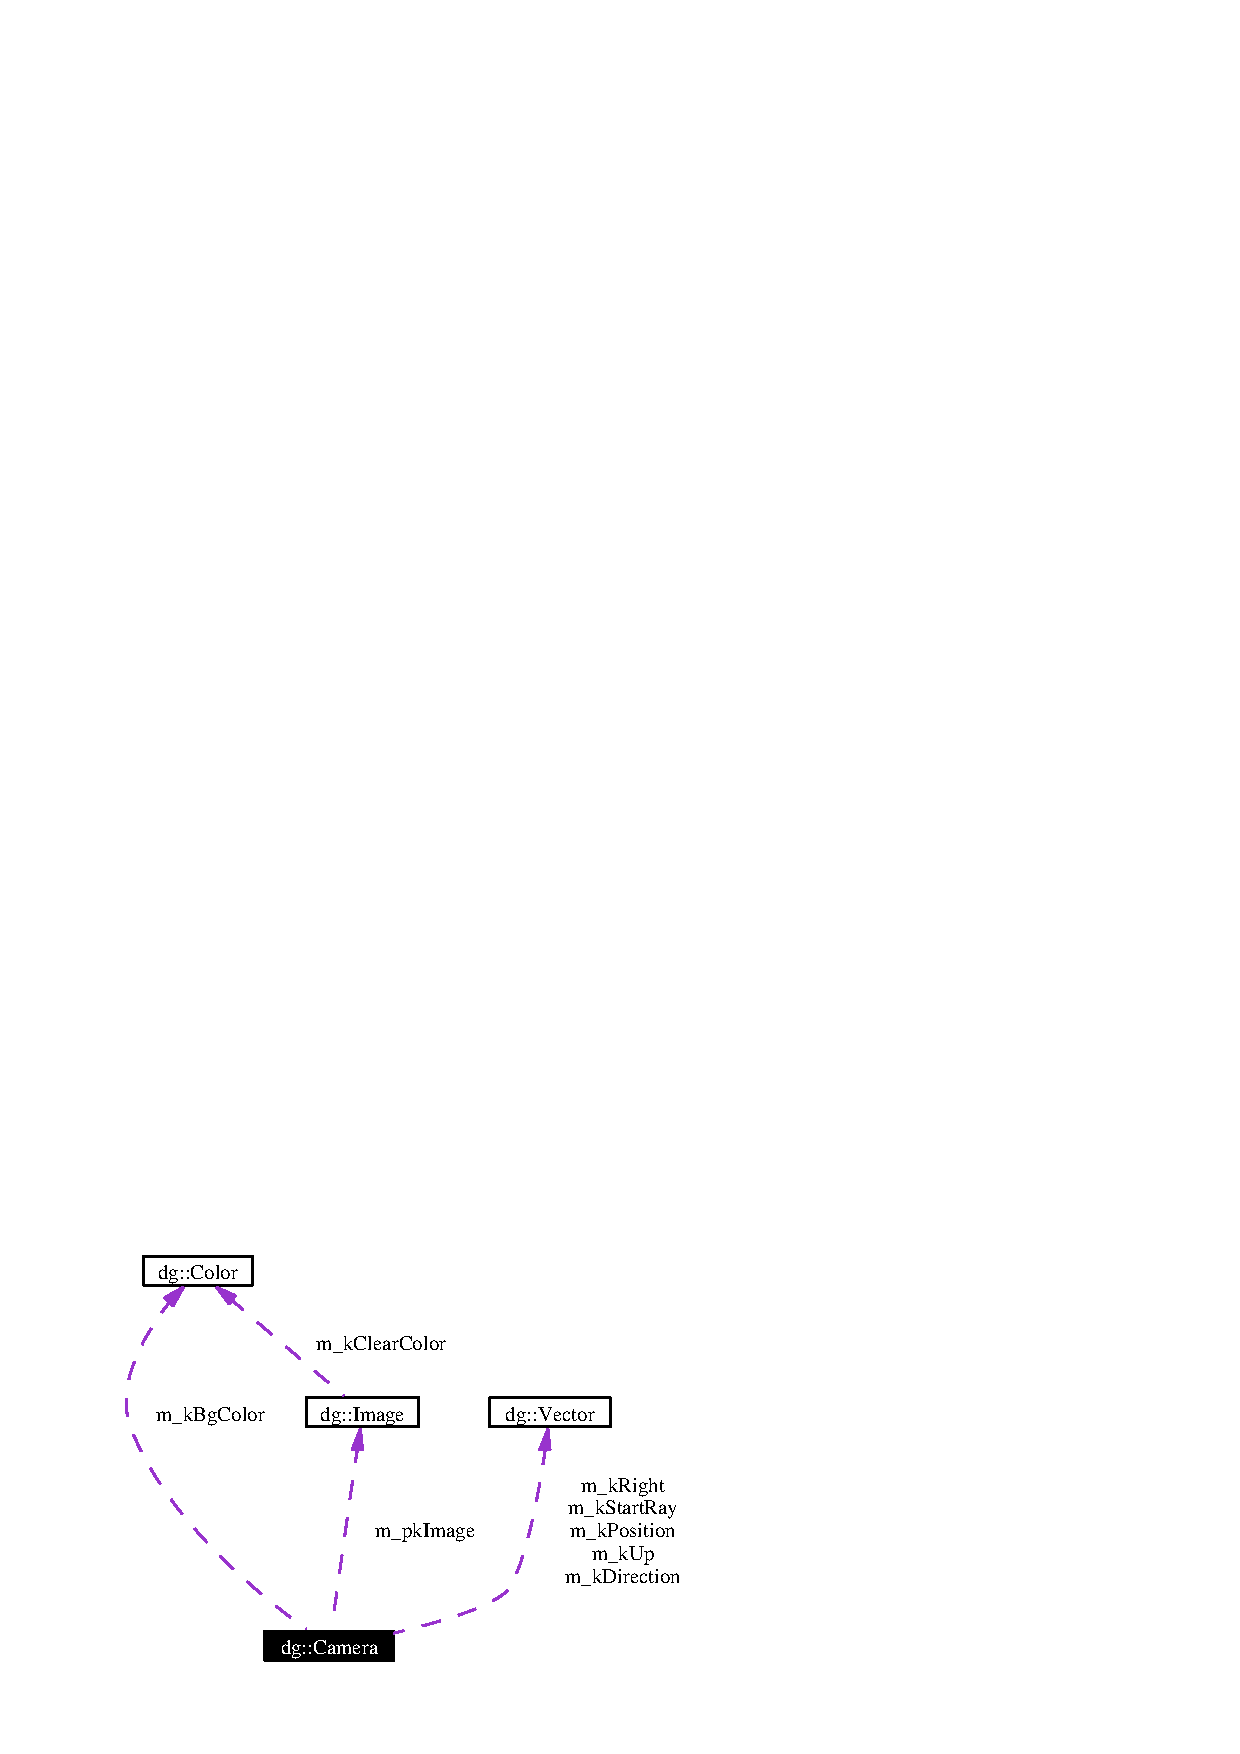
\includegraphics[width=172pt]{classdg_1_1Camera__coll__graph}
\end{center}
\end{figure}
\subsection*{Public Methods}
\begin{CompactItemize}
\item 
{\bf Camera} (const {\bf Vector} \&rk\-Pos={\bf Vector}(0.0f, 0.0f, 0.0f), const {\bf Vector} \&rk\-Dir={\bf Vector}(0.0f, 0.0f, 1.0f), const {\bf Vector} \&rk\-Up={\bf Vector}(0.0f, 1.0f, 0.0f), const {\bf Vector} \&rk\-Right={\bf Vector}(1.0f, 0.0f, 0.0f), {\bf Real} f\-Near=0.1f, {\bf Real} f\-Far=10.0f, {\bf Real} f\-Half\-Width=0.5f, {\bf Real} f\-Half\-Height=0.5f, {\bf Image} $\ast$pk\-Image=NULL)
\item 
{\bf $\sim$Camera} ()
\item 
void {\bf setup} ()
\item 
{\bf Vector} {\bf get\-Position} () const
\item 
void {\bf set\-Position} (const {\bf Vector} \&rk\-Position)
\item 
{\bf Vector} {\bf get\-Direction} () const
\item 
void {\bf set\-Direction} (const {\bf Vector} \&rk\-Direction)
\item 
{\bf Vector} {\bf get\-Up} () const
\item 
void {\bf set\-Up} (const {\bf Vector} \&rk\-Up)
\item 
{\bf Vector} {\bf get\-Right} () const
\item 
void {\bf set\-Right} (const {\bf Vector} \&rk\-Right)
\item 
void {\bf set\-Near} ({\bf Real} f\-Near)
\item 
{\bf Real} {\bf get\-Near} () const
\item 
void {\bf set\-Far} ({\bf Real} f\-Far)
\item 
{\bf Real} {\bf get\-Far} () const
\item 
void {\bf set\-Half\-Width} ({\bf Real} f\-Half\-Width)
\item 
{\bf Real} {\bf get\-Half\-Width} () const
\item 
void {\bf set\-Horizontal\-Fov} ({\bf Real} f\-Horiz\-Fov)
\item 
{\bf Real} {\bf get\-Horizontal\-Fov} () const
\item 
void {\bf set\-Half\-Height} ({\bf Real} f\-Half\-Height)
\item 
{\bf Real} {\bf get\-Half\-Height} () const
\item 
void {\bf set\-Vertical\-Fov} ({\bf Real} f\-Vert\-Fov)
\item 
{\bf Real} {\bf get\-Vertical\-Fov} () const
\item 
void {\bf set\-Background} (const {\bf Color} \&rk\-Color)
\item 
{\bf Color} {\bf get\-Background} () const
\item 
{\bf Vector} {\bf get\-Ray\-Dir} ({\bf UInt} ui\-X, {\bf UInt} ui\-Y) const
\item 
{\bf Vector} {\bf get\-Start\-Ray\-Dir} () const
\item 
void {\bf set\-Image} ({\bf Image} $\ast$pk\-Image)
\item 
const {\bf Image} $\ast$ {\bf get\-Image} () const
\item 
{\bf Image} $\ast$ {\bf get\-Image} ()
\item 
{\bf UInt} {\bf get\-Image\-Width} () const
\item 
{\bf UInt} {\bf get\-Image\-Height} () const
\item 
{\bf UInt} {\bf get\-Image\-Channels} () const
\item 
{\bf Real} {\bf get\-Pixel\-Width} () const
\item 
{\bf Real} {\bf get\-Pixel\-Height} () const
\end{CompactItemize}


\subsection{Constructor \& Destructor Documentation}
\index{dg::Camera@{dg::Camera}!Camera@{Camera}}
\index{Camera@{Camera}!dg::Camera@{dg::Camera}}
\subsubsection{\setlength{\rightskip}{0pt plus 5cm}Camera::Camera (const {\bf Vector} \& {\em rk\-Pos} = {\bf Vector}(0.0f, 0.0f, 0.0f), const {\bf Vector} \& {\em rk\-Dir} = {\bf Vector}(0.0f, 0.0f, 1.0f), const {\bf Vector} \& {\em rk\-Up} = {\bf Vector}(0.0f, 1.0f, 0.0f), const {\bf Vector} \& {\em rk\-Right} = {\bf Vector}(1.0f, 0.0f, 0.0f), {\bf Real} {\em f\-Near} = 0.1f, {\bf Real} {\em f\-Far} = 10.0f, {\bf Real} {\em f\-Half\-Width} = 0.5f, {\bf Real} {\em f\-Half\-Height} = 0.5f, {\bf Image} $\ast$ {\em pk\-Image} = NULL)}\label{classdg_1_1Camera_a0}




Definition at line 7 of file Camera.cpp.

References dg::Real.\index{dg::Camera@{dg::Camera}!~Camera@{$\sim$Camera}}
\index{~Camera@{$\sim$Camera}!dg::Camera@{dg::Camera}}
\subsubsection{\setlength{\rightskip}{0pt plus 5cm}Camera::$\sim$Camera ()}\label{classdg_1_1Camera_a1}




Definition at line 25 of file Camera.cpp.

\subsection{Member Function Documentation}
\index{dg::Camera@{dg::Camera}!getBackground@{getBackground}}
\index{getBackground@{getBackground}!dg::Camera@{dg::Camera}}
\subsubsection{\setlength{\rightskip}{0pt plus 5cm}{\bf Color} dg::Camera::get\-Background ()\hspace{0.3cm}{\tt  [inline]}}\label{classdg_1_1Camera_a24}




Definition at line 257 of file Camera.h.\index{dg::Camera@{dg::Camera}!getDirection@{getDirection}}
\index{getDirection@{getDirection}!dg::Camera@{dg::Camera}}
\subsubsection{\setlength{\rightskip}{0pt plus 5cm}{\bf Vector} dg::Camera::get\-Direction ()\hspace{0.3cm}{\tt  [inline]}}\label{classdg_1_1Camera_a5}




Definition at line 143 of file Camera.h.

Referenced by dg::Visualizer::draw\-Polygons(), dg::Visualizer::on\-Startup(), dg::Ray\-Tracer::render(), dg::Hypertexture::render(), dg::Visualizer::setup\-Camera(), and dg::Visualizer::setup\-Ray\-Tracer().\index{dg::Camera@{dg::Camera}!getFar@{getFar}}
\index{getFar@{getFar}!dg::Camera@{dg::Camera}}
\subsubsection{\setlength{\rightskip}{0pt plus 5cm}{\bf Real} dg::Camera::get\-Far ()\hspace{0.3cm}{\tt  [inline]}}\label{classdg_1_1Camera_a14}




Definition at line 183 of file Camera.h.

Referenced by dg::Ray\-Tracer::render(), and dg::Hypertexture::render().\index{dg::Camera@{dg::Camera}!getHalfHeight@{getHalfHeight}}
\index{getHalfHeight@{getHalfHeight}!dg::Camera@{dg::Camera}}
\subsubsection{\setlength{\rightskip}{0pt plus 5cm}{\bf Real} dg::Camera::get\-Half\-Height ()\hspace{0.3cm}{\tt  [inline]}}\label{classdg_1_1Camera_a20}




Definition at line 203 of file Camera.h.

Referenced by dg::Ray\-Tracer::render(), and dg::Hypertexture::render().\index{dg::Camera@{dg::Camera}!getHalfWidth@{getHalfWidth}}
\index{getHalfWidth@{getHalfWidth}!dg::Camera@{dg::Camera}}
\subsubsection{\setlength{\rightskip}{0pt plus 5cm}{\bf Real} dg::Camera::get\-Half\-Width ()\hspace{0.3cm}{\tt  [inline]}}\label{classdg_1_1Camera_a16}




Definition at line 193 of file Camera.h.

Referenced by dg::Ray\-Tracer::render(), and dg::Hypertexture::render().\index{dg::Camera@{dg::Camera}!getHorizontalFov@{getHorizontalFov}}
\index{getHorizontalFov@{getHorizontalFov}!dg::Camera@{dg::Camera}}
\subsubsection{\setlength{\rightskip}{0pt plus 5cm}{\bf Real} Camera::get\-Horizontal\-Fov ()\hspace{0.3cm}{\tt  [inline]}}\label{classdg_1_1Camera_a18}




Definition at line 35 of file Camera.cpp.

References dg::Arc\-Tangent(), dg::Degrees(), and dg::Real.\index{dg::Camera@{dg::Camera}!getImage@{getImage}}
\index{getImage@{getImage}!dg::Camera@{dg::Camera}}
\subsubsection{\setlength{\rightskip}{0pt plus 5cm}{\bf Image} $\ast$ dg::Camera::get\-Image ()\hspace{0.3cm}{\tt  [inline]}}\label{classdg_1_1Camera_a29}




Definition at line 247 of file Camera.h.\index{dg::Camera@{dg::Camera}!getImage@{getImage}}
\index{getImage@{getImage}!dg::Camera@{dg::Camera}}
\subsubsection{\setlength{\rightskip}{0pt plus 5cm}const {\bf Image} $\ast$ dg::Camera::get\-Image ()\hspace{0.3cm}{\tt  [inline]}}\label{classdg_1_1Camera_a28}




Definition at line 242 of file Camera.h.

Referenced by dg::Ray\-Tracer::render(), and dg::Hypertexture::render().\index{dg::Camera@{dg::Camera}!getImageChannels@{getImageChannels}}
\index{getImageChannels@{getImageChannels}!dg::Camera@{dg::Camera}}
\subsubsection{\setlength{\rightskip}{0pt plus 5cm}{\bf UInt} dg::Camera::get\-Image\-Channels ()\hspace{0.3cm}{\tt  [inline]}}\label{classdg_1_1Camera_a32}




Definition at line 229 of file Camera.h.\index{dg::Camera@{dg::Camera}!getImageHeight@{getImageHeight}}
\index{getImageHeight@{getImageHeight}!dg::Camera@{dg::Camera}}
\subsubsection{\setlength{\rightskip}{0pt plus 5cm}{\bf UInt} dg::Camera::get\-Image\-Height ()\hspace{0.3cm}{\tt  [inline]}}\label{classdg_1_1Camera_a31}




Definition at line 221 of file Camera.h.\index{dg::Camera@{dg::Camera}!getImageWidth@{getImageWidth}}
\index{getImageWidth@{getImageWidth}!dg::Camera@{dg::Camera}}
\subsubsection{\setlength{\rightskip}{0pt plus 5cm}{\bf UInt} dg::Camera::get\-Image\-Width ()\hspace{0.3cm}{\tt  [inline]}}\label{classdg_1_1Camera_a30}




Definition at line 213 of file Camera.h.\index{dg::Camera@{dg::Camera}!getNear@{getNear}}
\index{getNear@{getNear}!dg::Camera@{dg::Camera}}
\subsubsection{\setlength{\rightskip}{0pt plus 5cm}{\bf Real} dg::Camera::get\-Near ()\hspace{0.3cm}{\tt  [inline]}}\label{classdg_1_1Camera_a12}




Definition at line 173 of file Camera.h.

Referenced by dg::Ray\-Tracer::render(), and dg::Hypertexture::render().\index{dg::Camera@{dg::Camera}!getPixelHeight@{getPixelHeight}}
\index{getPixelHeight@{getPixelHeight}!dg::Camera@{dg::Camera}}
\subsubsection{\setlength{\rightskip}{0pt plus 5cm}{\bf Real} dg::Camera::get\-Pixel\-Height ()\hspace{0.3cm}{\tt  [inline]}}\label{classdg_1_1Camera_a34}




Definition at line 272 of file Camera.h.\index{dg::Camera@{dg::Camera}!getPixelWidth@{getPixelWidth}}
\index{getPixelWidth@{getPixelWidth}!dg::Camera@{dg::Camera}}
\subsubsection{\setlength{\rightskip}{0pt plus 5cm}{\bf Real} dg::Camera::get\-Pixel\-Width ()\hspace{0.3cm}{\tt  [inline]}}\label{classdg_1_1Camera_a33}




Definition at line 267 of file Camera.h.\index{dg::Camera@{dg::Camera}!getPosition@{getPosition}}
\index{getPosition@{getPosition}!dg::Camera@{dg::Camera}}
\subsubsection{\setlength{\rightskip}{0pt plus 5cm}{\bf Vector} dg::Camera::get\-Position ()\hspace{0.3cm}{\tt  [inline]}}\label{classdg_1_1Camera_a3}




Definition at line 133 of file Camera.h.

Referenced by dg::Visualizer::draw\-Polygons(), dg::Ray\-Tracer::render(), and dg::Visualizer::setup\-Camera().\index{dg::Camera@{dg::Camera}!getRayDir@{getRayDir}}
\index{getRayDir@{getRayDir}!dg::Camera@{dg::Camera}}
\subsubsection{\setlength{\rightskip}{0pt plus 5cm}{\bf Vector} Camera::get\-Ray\-Dir ({\bf UInt} {\em ui\-X}, {\bf UInt} {\em ui\-Y}) const}\label{classdg_1_1Camera_a25}




Definition at line 50 of file Camera.cpp.

References dg::Vector::normalize(), dg::UInt, dg::Vector::x(), dg::Vector::y(), and dg::Vector::z().\index{dg::Camera@{dg::Camera}!getRight@{getRight}}
\index{getRight@{getRight}!dg::Camera@{dg::Camera}}
\subsubsection{\setlength{\rightskip}{0pt plus 5cm}{\bf Vector} dg::Camera::get\-Right ()\hspace{0.3cm}{\tt  [inline]}}\label{classdg_1_1Camera_a9}




Definition at line 163 of file Camera.h.

Referenced by dg::Ray\-Tracer::render(), and dg::Hypertexture::render().\index{dg::Camera@{dg::Camera}!getStartRayDir@{getStartRayDir}}
\index{getStartRayDir@{getStartRayDir}!dg::Camera@{dg::Camera}}
\subsubsection{\setlength{\rightskip}{0pt plus 5cm}{\bf Vector} dg::Camera::get\-Start\-Ray\-Dir ()\hspace{0.3cm}{\tt  [inline]}}\label{classdg_1_1Camera_a26}




Definition at line 262 of file Camera.h.\index{dg::Camera@{dg::Camera}!getUp@{getUp}}
\index{getUp@{getUp}!dg::Camera@{dg::Camera}}
\subsubsection{\setlength{\rightskip}{0pt plus 5cm}{\bf Vector} dg::Camera::get\-Up ()\hspace{0.3cm}{\tt  [inline]}}\label{classdg_1_1Camera_a7}




Definition at line 153 of file Camera.h.

Referenced by dg::Visualizer::draw\-Polygons(), dg::Ray\-Tracer::render(), dg::Hypertexture::render(), and dg::Visualizer::setup\-Camera().\index{dg::Camera@{dg::Camera}!getVerticalFov@{getVerticalFov}}
\index{getVerticalFov@{getVerticalFov}!dg::Camera@{dg::Camera}}
\subsubsection{\setlength{\rightskip}{0pt plus 5cm}{\bf Real} Camera::get\-Vertical\-Fov ()\hspace{0.3cm}{\tt  [inline]}}\label{classdg_1_1Camera_a22}




Definition at line 45 of file Camera.cpp.

References dg::Arc\-Tangent(), dg::Degrees(), and dg::Real.\index{dg::Camera@{dg::Camera}!setBackground@{setBackground}}
\index{setBackground@{setBackground}!dg::Camera@{dg::Camera}}
\subsubsection{\setlength{\rightskip}{0pt plus 5cm}void dg::Camera::set\-Background (const {\bf Color} \& {\em rk\-Color})\hspace{0.3cm}{\tt  [inline]}}\label{classdg_1_1Camera_a23}




Definition at line 252 of file Camera.h.\index{dg::Camera@{dg::Camera}!setDirection@{setDirection}}
\index{setDirection@{setDirection}!dg::Camera@{dg::Camera}}
\subsubsection{\setlength{\rightskip}{0pt plus 5cm}void dg::Camera::set\-Direction (const {\bf Vector} \& {\em rk\-Direction})\hspace{0.3cm}{\tt  [inline]}}\label{classdg_1_1Camera_a6}




Definition at line 148 of file Camera.h.

Referenced by dg::Visualizer::setup\-Camera().\index{dg::Camera@{dg::Camera}!setFar@{setFar}}
\index{setFar@{setFar}!dg::Camera@{dg::Camera}}
\subsubsection{\setlength{\rightskip}{0pt plus 5cm}void dg::Camera::set\-Far ({\bf Real} {\em f\-Far})\hspace{0.3cm}{\tt  [inline]}}\label{classdg_1_1Camera_a13}




Definition at line 188 of file Camera.h.

Referenced by dg::Visualizer::setup\-Camera().\index{dg::Camera@{dg::Camera}!setHalfHeight@{setHalfHeight}}
\index{setHalfHeight@{setHalfHeight}!dg::Camera@{dg::Camera}}
\subsubsection{\setlength{\rightskip}{0pt plus 5cm}void dg::Camera::set\-Half\-Height ({\bf Real} {\em f\-Half\-Height})\hspace{0.3cm}{\tt  [inline]}}\label{classdg_1_1Camera_a19}




Definition at line 208 of file Camera.h.

Referenced by dg::Visualizer::setup\-Camera().\index{dg::Camera@{dg::Camera}!setHalfWidth@{setHalfWidth}}
\index{setHalfWidth@{setHalfWidth}!dg::Camera@{dg::Camera}}
\subsubsection{\setlength{\rightskip}{0pt plus 5cm}void dg::Camera::set\-Half\-Width ({\bf Real} {\em f\-Half\-Width})\hspace{0.3cm}{\tt  [inline]}}\label{classdg_1_1Camera_a15}




Definition at line 198 of file Camera.h.

Referenced by dg::Visualizer::setup\-Camera().\index{dg::Camera@{dg::Camera}!setHorizontalFov@{setHorizontalFov}}
\index{setHorizontalFov@{setHorizontalFov}!dg::Camera@{dg::Camera}}
\subsubsection{\setlength{\rightskip}{0pt plus 5cm}void Camera::set\-Horizontal\-Fov ({\bf Real} {\em f\-Horiz\-Fov})\hspace{0.3cm}{\tt  [inline]}}\label{classdg_1_1Camera_a17}




Definition at line 30 of file Camera.cpp.

References dg::Radians(), dg::Real, and dg::Tangent().\index{dg::Camera@{dg::Camera}!setImage@{setImage}}
\index{setImage@{setImage}!dg::Camera@{dg::Camera}}
\subsubsection{\setlength{\rightskip}{0pt plus 5cm}void dg::Camera::set\-Image ({\bf Image} $\ast$ {\em pk\-Image})\hspace{0.3cm}{\tt  [inline]}}\label{classdg_1_1Camera_a27}




Definition at line 237 of file Camera.h.

Referenced by dg::Visualizer::setup\-Hypertexture(), and dg::Visualizer::setup\-Ray\-Tracer().\index{dg::Camera@{dg::Camera}!setNear@{setNear}}
\index{setNear@{setNear}!dg::Camera@{dg::Camera}}
\subsubsection{\setlength{\rightskip}{0pt plus 5cm}void dg::Camera::set\-Near ({\bf Real} {\em f\-Near})\hspace{0.3cm}{\tt  [inline]}}\label{classdg_1_1Camera_a11}




Definition at line 178 of file Camera.h.

Referenced by dg::Visualizer::setup\-Camera().\index{dg::Camera@{dg::Camera}!setPosition@{setPosition}}
\index{setPosition@{setPosition}!dg::Camera@{dg::Camera}}
\subsubsection{\setlength{\rightskip}{0pt plus 5cm}void dg::Camera::set\-Position (const {\bf Vector} \& {\em rk\-Position})\hspace{0.3cm}{\tt  [inline]}}\label{classdg_1_1Camera_a4}




Definition at line 138 of file Camera.h.

Referenced by dg::Visualizer::setup\-Camera().\index{dg::Camera@{dg::Camera}!setRight@{setRight}}
\index{setRight@{setRight}!dg::Camera@{dg::Camera}}
\subsubsection{\setlength{\rightskip}{0pt plus 5cm}void dg::Camera::set\-Right (const {\bf Vector} \& {\em rk\-Right})\hspace{0.3cm}{\tt  [inline]}}\label{classdg_1_1Camera_a10}




Definition at line 168 of file Camera.h.

Referenced by dg::Visualizer::setup\-Camera().\index{dg::Camera@{dg::Camera}!setUp@{setUp}}
\index{setUp@{setUp}!dg::Camera@{dg::Camera}}
\subsubsection{\setlength{\rightskip}{0pt plus 5cm}void dg::Camera::set\-Up (const {\bf Vector} \& {\em rk\-Up})\hspace{0.3cm}{\tt  [inline]}}\label{classdg_1_1Camera_a8}




Definition at line 158 of file Camera.h.

Referenced by dg::Visualizer::setup\-Camera().\index{dg::Camera@{dg::Camera}!setup@{setup}}
\index{setup@{setup}!dg::Camera@{dg::Camera}}
\subsubsection{\setlength{\rightskip}{0pt plus 5cm}void Camera::setup ()}\label{classdg_1_1Camera_a2}




Definition at line 96 of file Camera.cpp.

References dg::Image::height(), dg::Real, dg::Image::width(), dg::Vector::x(), dg::Vector::y(), and dg::Vector::z().\index{dg::Camera@{dg::Camera}!setVerticalFov@{setVerticalFov}}
\index{setVerticalFov@{setVerticalFov}!dg::Camera@{dg::Camera}}
\subsubsection{\setlength{\rightskip}{0pt plus 5cm}void Camera::set\-Vertical\-Fov ({\bf Real} {\em f\-Vert\-Fov})\hspace{0.3cm}{\tt  [inline]}}\label{classdg_1_1Camera_a21}




Definition at line 40 of file Camera.cpp.

References dg::Radians(), dg::Real, and dg::Tangent().

The documentation for this class was generated from the following files:\begin{CompactItemize}
\item 
{\bf Camera.h}\item 
{\bf Camera.cpp}\end{CompactItemize}
